%\documentclass[preprint,groupeaddress]{revtex4}
\documentclass[twocolumn,superscriptaddress]{revtex4}


\usepackage{amsmath} 
\usepackage{amssymb} 
 \usepackage{amsfonts}

\usepackage{graphicx} 

\usepackage{array}
\usepackage{multirow}
\usepackage{color}
\usepackage{transparent}
\usepackage{float}

\newcommand{\vect}[1]{\boldsymbol{\mathbf{#1}}}



\begin{document}
\bibliographystyle{apsrev4-1} 

\title{Diffusion-Controlled Reactions over Fluctuating Barriers} 

\author{Jakob J. Kolb}
\affiliation{Department of Physics, Humboldt Universit{\"a}t zu Berlin, Newtonstr. 15, 12489 Berlin, Germany, Germany}
\author{Stefano Angioletti-Uberti}
\affiliation{Department of Physics, Humboldt Universit{\"a}t zu Berlin, Newtonstr. 15, 12489 Berlin, Germany, Germany}
\author{Joachim Dzubiella}
%\thanks{To whom correspondence should be addressed. E-mail: joachim.dzubiella@helmholtz-berlin.de}
\affiliation{Department of Physics, Humboldt Universit{\"a}t zu Berlin, Newtonstr. 15, 12489 Berlin, Germany, Germany}
\affiliation{Soft Matter and Functional Materials, Helmholtz-Center Berlin, Hahn-Meitner Platz 1, 14109 Berlin, Germany}



\begin{abstract}
Recent studies on tunable nano-reactors with a thermosensitive polymer shell have shown curious effects in reaction rates
right at the polymer critical solution temperature.
The shell is presumably stochastically fluctuating between states with different permeability for the substrate.
To investigate this effect a simplified system of diffusing particles in the vicinity of a spherical sink shielded by a metastable potential barrier is investigated. We derive an implicit solution for the resulting Fokker-Planck equation to obtain the diffusion-controlled reaction rate and verify these results with Brownian dynamics computer simulations. The system shows resonant activation as previously seen with thermally activated escape over fluctuating barriers.


\end{abstract}

\maketitle

\section{Introduction}


\begin{figure}[H]
    \input{plots/tSkizzeSmall.eps_tex}
    \caption{Sketch of the system consisting of sink and fluctuating barrier. Sink radius is $R_s$, gap between sink and Barrier is of with $l$ and barrier width is $g\cdot l$. Barrier transition rates between states $U_0$ and $U_1$ are $\gamma_{01}, \gamma_{10}$.}
\label{fig0}
\end{figure}


\section{Methods} We study the problem of diffusion limited reaction rates in the Smoluchowski Debye sense \cite{Smoluchowski1917a, Debye1942} in the presence of a fluctuating boxcar shaped potential barrier. The barrier switches between different states according to a discrete time reversible Markov process $\eta(t)$. Therefore the system evolution follows the following stochastic differential equation
\begin{equation}
    \frac{{\rm d} \vec{r}}{{\rm d} t} = \vec{\nabla}\frac{1}{\gamma}f(r)\eta(t) + \sqrt{2D}\vec{\varepsilon}(t)
    \label{SDE}
\end{equation}
where $\varepsilon(t)$ is white Gaussian noise with time correlation $\left< \varepsilon(t) \varepsilon(t') \right> = \delta(t-t')$ and $\eta(t) \in [U_0, U_1,\cdots U_n]$ and $f(r) = \Theta(r-a)-\Theta(r-b)$ define the hight and shape of the potential barrier. The intervals in $r$ with constant potential namely $R_s \le r < a$, $a \le r < b$ and $b\le r$ will be referred to as $(I)$, $(II)$ and $(III)$ in the following.\\
For the Brownian particles it is assumed that their total density equals one at $r \rightarrow \infty$ and that they vanish as their trajectory crosses the boundary of the sink at $r = R_s$. It is therefore appropriate to normalize the PDF of the system not to unity but to the number of particles per volume. \\
Now, equivalently to the SDE the system can be described in terms of a combined reaction-diffusion equation for the particle density function $\rho_n(\vec{r},t)$ of the discrete variable $n$ of the potential and the continuous variable $\vec{r}$ of the overdamped particles
\begin{equation}
    \frac{\partial}{\partial t}\vect{\rho}(\vec{r},t) = \left\{ \mathbb{F} + \mathbb{W} \right\} \vect{\rho}(\vec{r},t)
    \label{mfpe}
\end{equation}
with $\mathbb{F}$ being the Fokker-Planck operator
\begin{equation}
    \mathbb{F} = {\rm  diag}\left[\vec{\nabla} \frac{1}{\gamma} \left(\vec{\nabla} U_n f(r)\right) + D\vec{\nabla}^{2} \right].
    \label{FPO}
\end{equation}
$\mathbb{W}$ is the transition rate matrix of the Markov process for the barrier switching. $\vect{\rho}(\vec{r},t)=(\rho_0(\vec{r},t),\cdots,\rho_n(\vec{r},t))^{T}$ denotes the vector of particle density functions related to each state of the potential barrier. Since the underlying Markov process of $\mathbb{W}$ is time reversible the transition rate matrix satisfies detailed balance.This also implies that the particle density vector at infinity is equal to the equilibrium distribution $\vect{\rho}^{(eq)}$ of $\mathbb{W}$. \\
Therefore it is possible to find a similarity transform $\mathbb{T}_{ij}=[\rho_i^{(eq)}]^{1/2}\delta_{i,j}$ such that the resulting $\mathbb{T}^{-1}\mathbb{W}\mathbb{T} = \mathbb{S}$ is symmetric \cite{Oppenheim1977}. This symmetric matrix can then be diagonalized by an orthogonal transformation $\mathbb{D}$ resulting in $\mathbb{D}^{\dagger}\mathbb{S}\mathbb{D} = - {\rm diag}[\lambda_n]$. It can be shown \cite{VanKampen1992} that $\lambda_{i>0}>0$ and $\lambda_0=0$ with corresponding eigenvector $\mathbb{D}_{0,i}=[\rho_i^{(eq)}]^{1/2}$.  \\
Now we can give a steady state solution to eq. \eqref{mfpe} in terms of eigenfunctions of $\mathbb{W}$
\begin{align}
    \label{solution}
    \tilde{\rho}_{1}^{(j)}(r) &= c_{1,1}^{(j)} + c_{1,2}^{(j)} \frac{1}{r} \\
    \tilde{\rho}_{n \ne 1}^{(j)}(r) &= c_{n,1}^{(j)}\frac{1}{r} \exp\left[-r\sqrt{\frac{\lambda_n}{D}}\right] + c_{n,2}^{(j)}\frac{1}{r} \exp\left[r\sqrt{\frac{\lambda_n}{D}}\right]  \nonumber
\end{align}
separately for the regions $(I)$, $(II)$ and $(III)$ exploiting the fact that the Fokker-Planck operator $\mathbb{F}$ is invariant under the tranfsormations $\mathbb{T}$ and $\mathbb{D}$ for $r\ne a, b$. The coefficients $c^{(j)}_{n,k}$ have to be obtained from boundary and fitting conditions at $r=a,b$. From this solution it is visible that the spacial influence of the potential fluctuations decays with a certain \textit{decay length} equal to
\begin{equation}
    r_d = \left\{\sqrt{\frac{\lambda_m}{D}}\right\}^{-1}
    \label{decay_length}
\end{equation}
that only depends on the diffusion constant of the Brownian particles and the largest nonzero eigenvalue of the transition matrix $\lambda_m$.\\
To derive these fitting conditions we use eq. \eqref{mfpe} which in steady state is equivalent to
\begin{equation*}
     \frac{1}{\gamma}\rho_n(r) \vec{\nabla} U_n(r) + D \vec{\nabla} \rho_n(r) = \frac{J_n(R_s)}{4 \pi} - \left\{ \mathbb{W} \int_{R_s}^{r} \vect{\rho}(r') {\rm d} r' \right\}_{n}
\end{equation*}
where $J_n$ denotes the flux of particles in state $n$ through the sink surface. This expression is then integrated over a small vicinity of size $\varepsilon$ including the jump discontinuity at $r = a$. Taking the limit of $\varepsilon \rightarrow 0$ results in 
\begin{equation}
    \vect{\rho}^{(I)}(a) = {\rm diag}\left[\exp\left\{\frac{U_n}{K_B T} \right\}\right]\vect{\rho}^{(II)}(a)
    \label{dens_fit1}
\end{equation}
where $\vect{\rho}^{(I)}(a)$ is the density profile for $r \le a$ and $\vect{\rho}^{(II)}(a)$ is the density profile for $ a<r\le b$ right at the jump discontinuity of the potential barrier (consequently $\vect{\rho}^{(III)}$ denotes the density profile at $b<r$). Analogous considerations lead to fitting conditions for the derivative of the density profile
\begin{equation}
    \vec{\nabla}\vect{\rho}^{(I)}(a) =\vec{\nabla}\vect{\rho}^{(II)}(a) 
    \label{dens_fit2}
\end{equation}
and to fitting conditions for the density profile and its derivative at the second jump discontinuity of the potential.
The coefficients $c_{n,i}^{(j)}$ in eq. \eqref{solution} are calculated by applying the inverse transform $\vect{\rho}(r) = \mathbb{D}^{\dagger}\mathbb{T}^{-1}\tilde{\vect{\rho}}(r)$ and solving the system of linear equations arising from the fit conditions in eq. \eqref{dens_fit1}, \eqref{dens_fit2} and boundary conditions at $r=R_s$ and $r \rightarrow \infty$. Finally, the diffusion controlled reaction rate over the fluctuating barrier is calculated from $\vect{\rho}^{(I)}$ as
\begin{equation}
    k = 4 \pi D R_s^{2}\sum_n \left. \frac{\partial \rho_n^{(I)}(r)}{\partial r} \right|_{R_s}
    \label{rate_konstant}
\end{equation}
\section{Results and Discussion}
We consider the most simple model to illustrate some basic features of the model. Therefore we set $U_0$ to zero and vary only $U_1$. Furthermore, we take the transition rates between these states to be symmetric i.e. $\gamma_{01}=\gamma_{10}$.
For this simplified system we calculate the radial steady state density profiles resulting from the reverse transform of eqs. \eqref{solution} and the solution of the system of linear equations for the remaining coefficients.
\begin{figure}[H]
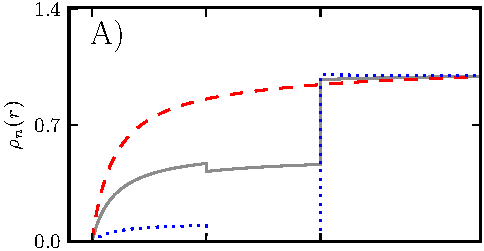
\includegraphics[width= .45 \textwidth]{plots/d1.pdf}
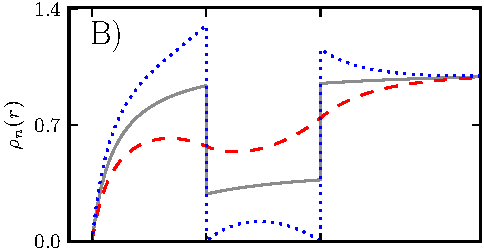
\includegraphics[width= .45 \textwidth]{plots/d2.pdf}
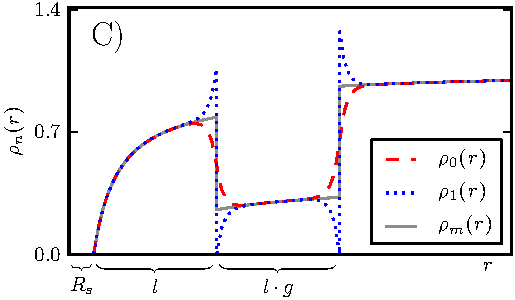
\includegraphics[width= .45 \textwidth]{plots/d3.pdf}
\caption{Steady state density profiles $\rho_0, \rho_1$ for states $U_0, U_1$ of the barrier and mean density profile $\rho_m$ vs. distance from center of sink. All parameters but decay length are fixed: $l=5$, $g=1$, $U_1 = 10 K_B T, U_0 = 0$ are constant and decay length is A) $r_d = 20$, B) $r_d=2$, and C) $r_d=0.5$. \emph{Density profiles strongly depend on the decay length.}}
\label{fig1}
\end{figure}
It becomes obvious, that for a certain value of the decay length comparable to the barrier dimensions the density inside the barrier is considerably higher that what is is for decay lengths far off. This is also directly reflected in the resulting reaction rates. For a certain decay length depending on the barrier spacing the reaction rate takes a maximum value. This phenomenon has previously been observed in escape over fluctuating barriers where a minimum in mean first passage times of trapped particles over a fluctuating barrier is known as \emph{Resonant Activation}.
\begin{figure}[H]
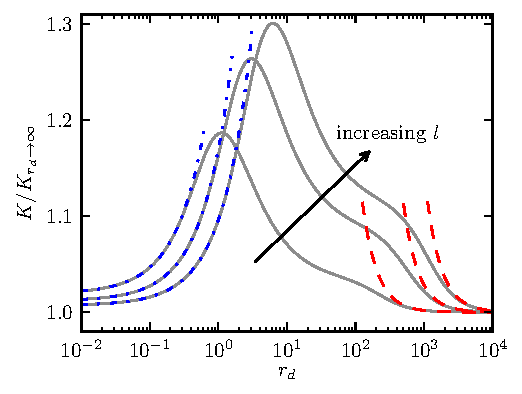
\includegraphics[width= .5 \textwidth]{plots/ab_rates.pdf}
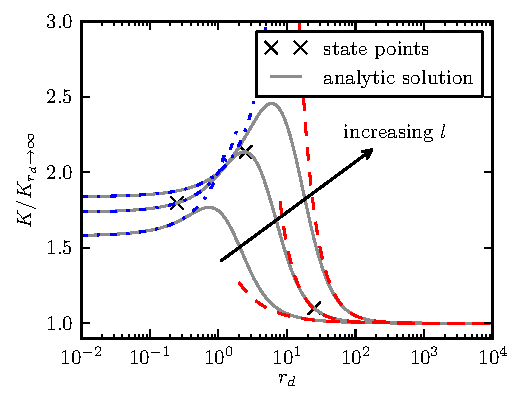
\includegraphics[width= .5 \textwidth]{plots/rb_rates.pdf}
\caption{normalized absorption rate vs. decay length for attractive and repulsive fluctuating barrier. \newline Parameters are $U_1 = \pm 10 K_B T, U_0= 0, g = 1$ and $l=2,5,10$. Approximation for very fast and very slow barrier fluctuations are depicted by dashed blue and red lines respectively. State points from the density profiles are marked by black crosses. \emph{The resonance effect increases with barrier spacing}.}
\label{fig3}
\end{figure}
The limits in fig \ref{fig3} can be derived from the full solution of for the absorption rate by means of ether a Taylor expansion in the case of the $r_d \gg 1$ case or by reducing nominator and denominator separately to leading orders in the $r_d \ll 1$ case. The slow fluctuation i.e. long decay limit can treated by standard Debye theory. In this case one half of the Brownian particles move subject to the potential in one state respectively with no switching possible. Then the total rate is the average of the rates over the stable barriers in each state. In the fast fluctuation i.e. short decay limit the changes in the reaction coordinate are much faster that the changes in the spatial coordinate. Therefore the Brownian particles will move subject to a mean potential barrier. This limit can then again be calculated by means of standard Debye theory.\\ Note that this limit is \emph{not} part of the solution we obtained. This is due to the fact, that the order of the limits from smooth to step potential and from finite to infinite switching rates is not arbitrary. This is illustrated by the comparison of results from numeric integration of the reaction rate over a barrier of shape
\begin{equation}
    U_n(r) = U_n \exp \left[- \left(\frac{r-R_s-l(1+g/2)}{gl}\right)^{n} \right] 
    \label{generalized_gaussian}
\end{equation}
compared to the solution of the $n \rightarrow \infty$ solution of the boxcar potential.
\begin{figure}[H]
    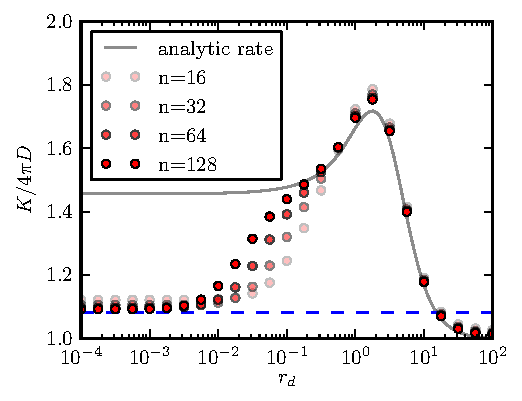
\includegraphics[width= 0.5 \textwidth]{plots/rates_for_barrier_transition.pdf}
    \caption{Results from numeric integration with repulsive generalized Gaussian potential barrier vs. analytic results from step potential. Debye rate for average boxcar potential marked blue. \emph{For smooth potentials in fast switching limit the Rate is that over an average potential barrier}.}
\end{figure}
The solution for the step potential is a valid approximation of smooth potentials when the switching rate and diffusion constant are such that the decay length $r_d$ is larger than the length scale of potential variations. If the differences in the particle densities in different states decay much faster than the potential changes the system can be described by Debye theory for an average potential barrier. 

\section{Concluding Remarks}

\acknowledgments
The authors thank the Alexander von Humboldt (AvH) Foundation and the Deutsche Forschungsgemeinschaft (DFG) 
for financial support. 

\bibliography{PRL.bib}

\end{document}
